% !TeX root = ./thesis.tex
% !TeX spellcheck = hu_HU
% !TeX encoding = UTF-8
% !TeX program = pdflatex
% !BIB program = bibtex
%TODO Change language to en_GB (recommended) or en_US for English documents
\documentclass[12pt,a4paper,oneside]{report}             % Egyoldalas (javasolt)
%\documentclass[11pt,a4paper,twoside,openright]{report}  % Duplex
\usepackage{setspace}
\usepackage{ listings }
\usepackage{float}
\usepackage[final]{pdfpages}
\usepackage[export]{adjustbox}
\usepackage{fancyhdr}

\input{include/packages}

\makeatletter
    \setlength\@fptop{0\p@}
\makeatother


%TODO Saját adataiddal töltsd ki a kommentek szerint
%--------------------------------------------------------------------------------------
\newcommand{\szerzoVezeteknev}{Tóth}
\newcommand{\szerzoKeresztnev}{Róbert}
\newcommand{\szerzoNeptun}{FBRENL}

\newcommand{\szakirany}{\merninf{}} % automat vagy infokom

\newcommand{\konzulensAMegszolitas}{Dr.}
\newcommand{\konzulensAVezeteknev}{Kranko}
\newcommand{\konzulensAKeresztnev}{Melinda}
\newcommand{\konzulensBMegszolitas}{}
\newcommand{\konzulensBVezeteknev}{}
\newcommand{\konzulensBKeresztnev}{}
\newcommand{\konzulensCMegszolitas}{}
\newcommand{\konzulensCVezeteknev}{}
\newcommand{\konzulensCKeresztnev}{}

\newcommand{\cim}{Mérnökinformatikus BSc} % Cím
\newcommand{\tanszek}{\szeint} % automatizálási (\szeaut) vagy távközlési (\szetat)
\newcommand{\doktipus}{\szakdolgozat} % Dokumentum típusa (\szakdolgozat, \diplomaterv vagy \dolgozat)
\newcommand{\szak}{\minfBSc}
\newcommand{\szakma}{\minfMSc}
 % villamosmérnöki msc (\villMSc) vagy villamosmérnöki bsc (\villBSc)
%TODO Nyelv beállítása
% Beállítások magyar nyelvű dolgozathoz
%--------------------------------------------------------------------------------------
% Elnevezések
%--------------------------------------------------------------------------------------
\newcommand{\sze}{Széchenyi István Egyetem}
\newcommand{\kvik}{Gépészmérnöki, Informatikai és Villamosmérnöki Kar}
\newcommand{\szeaut}{Automatizálási Tanszék}
\newcommand{\szetat}{Távközlési Tanszék}
\newcommand{\szeint}{Informatika Tanszék}

\newcommand{\aut}{Automatizálási Szakirány}
\newcommand{\infokom}{Infokommunikáció Szakirány}
\newcommand{\merninf}{Mérnökinformatikus Szakirány}

\newcommand{\keszitette}{Készítette}
\newcommand{\konzulens}{Konzulens}

\newcommand{\szakdolgozat}{Szakmai gyakorlati beszámoló}
\newcommand{\diplomaterv}{Diplomaterv}
\newcommand{\dolgozat}{Dolgozat}

\newcommand{\villBSc}{Villamosmérnöki BSc}
\newcommand{\minfBSc}{Szakmai gyakorlat ideje:}
\newcommand{\minfMSc}{2022.06.20 - 2022.08.19}

\newcommand{\pelda}{Példa}
\newcommand{\definicio}{Definíció}
\newcommand{\tetel}{Tétel}

\newcommand{\bevezetes}{Bevezetés}
\newcommand{\koszonetnyilvanitas}{Köszönetnyilvánítás}
\newcommand{\fuggelek}{Függelék}

% Opcionálisan átnevezhető címek
%\addto\captionsmagyar{%
%\renewcommand{\listfigurename}{Saját ábrajegyzék cím}
%\renewcommand{\listtablename}{Saját táblázatjegyzék cím}
%\renewcommand{\bibname}{Saját irodalomjegyzék név}
%}


\newcommand{\szerzo}{\szerzoVezeteknev{} \szerzoKeresztnev}
\newcommand{\konzulensA}{\konzulensAMegszolitas\konzulensAVezeteknev{} \konzulensAKeresztnev}
\newcommand{\konzulensB}{\konzulensBMegszolitas\konzulensBVezeteknev{} \konzulensBKeresztnev}
\newcommand{\konzulensC}{\konzulensCMegszolitas\konzulensCVezeteknev{} \konzulensCKeresztnev}

\newcommand{\selectthesislanguage}{\selecthungarian}

\bibliographystyle{huplain}

\def\lstlistingname{lista}

\newcommand{\appendixnumber}{6}  % a fofejezet-szamlalo az angol ABC 6. betuje (F) lesz

% Settings for English documents
%%--------------------------------------------------------------------------------------
% Elnevezések
%--------------------------------------------------------------------------------------
\newcommand{\sze}{Széchenyi István University}
\newcommand{\kvik}{Faculty of Mechanical Engineering, Informatics and Electrical Engineering}
\newcommand{\szeaut}{Department of Automation}
\newcommand{\szetat}{Department of Telecommunications}
\newcommand{\szeint}{Department of Computer Science}

\newcommand{\aut}{Specialization in Automation}
\newcommand{\infokom}{Specialization in Infocommunication}
\newcommand{\merninf}{Specialization in Computer Science Engineering}

\newcommand{\keszitette}{Author}
\newcommand{\konzulens}{Advisor}

\newcommand{\szakdolgozat}{Bachelor's Thesis}
\newcommand{\diplomaterv}{Master's Thesis}
\newcommand{\dolgozat}{Project} % TODO not the best word for this

\newcommand{\villBSc}{Electrical Engineering BSc}
\newcommand{\villMSc}{Electrical Engineering MSc}
\newcommand{\minfBSc}{Computer Science Engineering BSc}

\newcommand{\pelda}{Example}
\newcommand{\definicio}{Definition}
\newcommand{\tetel}{Theorem}

\newcommand{\bevezetes}{Introduction}
\newcommand{\koszonetnyilvanitas}{Acknowledgements}
\newcommand{\fuggelek}{Appendix}

% Optional custom titles
%\addto\captionsenglish{%
%\renewcommand*{\listfigurename}{Your list of figures title}
%\renewcommand*{\listtablename}{Your list of tables title}
%\renewcommand*{\bibname}{Your bibliography title}
%}


\newcommand{\szerzo}{\szerzoKeresztnev{} \szerzoVezeteknev}
\newcommand{\konzulensA}{\konzulensAMegszolitas\konzulensAKeresztnev{} \konzulensAVezeteknev}
\newcommand{\konzulensB}{\konzulensBMegszolitas\konzulensBKeresztnev{} \konzulensBVezeteknev}
\newcommand{\konzulensC}{\konzulensCMegszolitas\konzulensCKeresztnev{} \konzulensCVezeteknev}

\newcommand{\selectthesislanguage}{\selectenglish}

\bibliographystyle{plainnat}

\newcommand{\ie}{i.e.\@\xspace}
\newcommand{\Ie}{I.e.\@\xspace}
\newcommand{\eg}{e.g.\@\xspace}
\newcommand{\Eg}{E.g.\@\xspace}
\newcommand{\etal}{et al.\@\xspace}
\newcommand{\etc}{etc.\@\xspace}
\newcommand{\vs}{vs.\@\xspace}
\newcommand{\viz}{viz.\@\xspace} % videlicet
\newcommand{\cf}{cf.\@\xspace} % confer
\newcommand{\Cf}{Cf.\@\xspace}
\newcommand{\wrt}{w.r.t.\@\xspace} % with respect to

\newcommand{\appendixnumber}{1}  % a fofejezet-szamlalo az angol ABC 1. betuje (A) lesz



\newcommand{\szerzoMeta}{\szerzoVezeteknev{} \szerzoKeresztnev} % egy szerző esetén TODO@FMA két szerző
\input{include/preamble} % beállítások, nem kell vele foglalkoznod remélhetőleg, de ha valami latex hekkelésre vagy új parancsra van szükséged annak itt a helye


%--------------------------------------------------------------------------------------
% Itt kezdődik a dolgozat
%--------------------------------------------------------------------------------------
\begin{document}
\onehalfspacing

%TODO Feladatkiíró lap helye, csak a nyomtatott verzijóba kerül az eredeti példány
%~~~~~~~~~~~~~~~~~~~~~~~~~~~~~~~~~~~~~~~~~~~~~~~~~~~~~~~~~~~~~~~~~~~~~~~~~~~~~~~~~~~~~~
%\pagenumbering{gobble}
%--------------------------------------------------------------------------------------
% Feladatkiiras (a tanszeken atveheto, kinyomtatott valtozat)
%--------------------------------------------------------------------------------------
\clearpage
\begin{center}
\large
\textbf{FELADATKIÍRÁS}\\
\end{center}

A feladatkiíró lapot két példányban kell leadni a tanszéki adminisztrációban. Beadás előtt az egyiket visszakapod és a leadott munkába eredeti, tanszéki pecséttel ellátott és a tanszékvezető által aláírt lapot kell belefűzni (ezen oldal \emph{helyett}, ez az oldal csak útmutatás). Az elektronikusan feltöltött dolgozatban (tehát a könyvtár honlapjára feltöltött változatba) már nem kell beleszerkeszteni ezt a feladatkiírást.




% Címoldal
%~~~~~~~~~~~~~~~~~~~~~~~~~~~~~~~~~~~~~~~~~~~~~~~~~~~~~~~~~~~~~~~~~~~~~~~~~~~~~~~~~~~~~~
\hypersetup{pageanchor=false}
%--------------------------------------------------------------------------------------
%	The title page
%--------------------------------------------------------------------------------------
\begin{titlepage}
\begin{center}

\begin{figure}[!htb]
	\begin{minipage}{0.48\textwidth}
	  \centering
	  \hspace{-2cm}\includegraphics[width=70mm,keepaspectratio]{figures/infologo_2020_department.png}
	\end{minipage}\hfill
	\begin{minipage}{0.48\textwidth}
	  \centering
	  \hspace{-2cm}\includegraphics[width=70mm,keepaspectratio]{figures/infologo_2020_university.png}
	\end{minipage}
 \end{figure}
 

\vspace{100pt} %because it's the top
{\Huge \bfseries \MakeUppercase {\doktipus}}\\
\vspace{68pt}
{\huge \bfseries{\szerzo}}\\
\vspace{100pt}
{\huge \bfseries \cim}


\vspace{80pt}
\Large \textbf{\szak{}}\\
\Large \textbf{\szakma{}}\\

\vfill

\end{center}
\end{titlepage}
\hypersetup{pageanchor=false}



% Tartalomjegyzék
%~~~~~~~~~~~~~~~~~~~~~~~~~~~~~~~~~~~~~~~~~~~~~~~~~~~~~~~~~~~~~~~~~~~~~~~~~~~~~~~~~~~~~~
%\tableofcontents\vfill
%\addtocontents{toc}{\protect\thispagestyle{empty}}

% Ábrák listája - a word-ös sablon szerint szükséges
%~~~~~~~~~~~~~~~~~~~~~~~~~~~~~~~~~~~~~~~~~~~~~~~~~~~~~~~~~~~~~~~~~~~~~~~~~~~~~~~~~~~~~~
%\clearpage\phantomsection
%\listoffigures
%\addcontentsline{toc}{chapter}{\listfigurename}

% Nyilatkozat és Kivonat
%~~~~~~~~~~~~~~~~~~~~~~~~~~~~~~~~~~~~~~~~~~~~~~~~~~~~~~~~~~~~~~~~~~~~~~~~~~~~~~~~~~~~~~
%\selectlanguage{magyar}
\pagenumbering{gobble}
%--------------------------------------------------------------------------------------
% Nyilatkozat
%--------------------------------------------------------------------------------------
\begin{center}
\large
\textbf{Nyilatkozat}\\
\end{center}

\noindent
Alulírott, \textbf{\szerzoVezeteknev{} \szerzoKeresztnev{} (\szerzoNeptun)}, \szak{} szakos hallgató kijelentem, hogy a \textit{\cim} című \MakeLowercase{\doktipus{}} feladat kidolgozása a saját munkám, abban csak a megjelölt forrásokat, és a megjelölt mértékben használtam fel, az idézés szabályainak megfelelően, a hivatkozások pontos megjelölésével.

\setlength\parskip{\baselineskip}

\noindent
Eredményeim saját munkán, számításokon, kutatáson, valós méréseken alapulnak, és a legjobb tudásom szerint hitelesek.

\vspace*{24pt}
\begin{multicols}{2}
	\noindent
	Győr, \today

	\columnbreak
	\noindent
	\makebox[7cm][c]{\rule{6cm}{.4pt}}\\
	\makebox[7cm][c]{\emph{\szerzoVezeteknev{} \szerzoKeresztnev}}\\
	\makebox[7cm]{hallgató}
\end{multicols}

\thispagestyle{empty}

\vfill
\clearpage
\thispagestyle{empty} % an empty page

\selectthesislanguage
 % ez legenerálódik magától a fentebb megadott adatok alapján
%\include{content/abstract} %TODO ezt át kell írnod


% A dolgozat lényegi része
%~~~~~~~~~~~~~~~~~~~~~~~~~~~~~~~~~~~~~~~~~~~~~~~~~~~~~~~~~~~~~~~~~~~~~~~~~~~~~~~~~~~~~~
\pagenumbering{arabic}

%TODO készítsd el a saját munkád
\includepdf{tr_vallalat_igazolas.pdf}
\section*{\bevezetes}

A beszámolóban ismertetem a szakmai gyakorlatom során végzett munkámat, bemutatásra kerül maga az Attrecto Zrt., ahol a gyakorlatomat végeztem, ismertetem a gyakornoki idő alatt rámbízott feladatokat, a kollégákat, akikkel együtt dolgoztam és a tapasztalataimat.
\par A következő fejezetekben először áttekintést nyújtok a vállalatról, majd ismertetem a szerepemet és a projekteket, amelyeken dolgoztam.

\section*{Attrecto Zrt.}
\begin{figure}[H]
    \centering
    \includegraphics[width= 100mm]{figures/Attrecto_logo.png}
\end{figure}
\par Az Attrecto Zrt-t 2010-ben alapította három fiatal győri szoftverfejlesztő. A cég megalakulása óta professzionális mobil- és webfejlesztést és tanácsadást nyújt az ország legnagyobb cégeinek, valamint az Egyesült Államokban, Norvégiában és Ausztráliában működő ügyfeleknek. 

\par A jelenleg 85 főt foglalkoztató vállalat 2021-ben mintegy 900 millió forint árbevételt ért el. A vállalkozások számára végzett frontend-fejlesztés a fő területük, de számos iparági céggel dolgoznak együtt. A cég alapítása óta Közép-Európában ismert vállalkozássá vált. Ismertségét nemzetközi piacokon elért sikerei is alátámasztják, mint például a norvég Telenor számára fejlesztett mobilalkalmazás, vagy az Egyesült Államokban régóta végzett munkájuk. A vállalat a Financial Times 1000 leggyorsabban növekvő vállalat listáján és a Deloitte Fast Tech 500 leggyorsabban növekvő európai technológiai vállalat listáján is szerepel.
\pagenumbering{gobble}

A legmodernebb technológiák felhasználásával készítik a legkorszerűbb alkalmazásokat és a hozzájuk kapcsolódó szerveroldali megoldásokat. Többnyire átláthatóan, rugalmasan és hatékonyan dolgoznak az agilis szoftverfejlesztési módszertan alkalmazásával, és ügyfeleiket digitális példaképpé formálják az adott iparágban.
\par A vállalat jó kapcsolatot ápol a győri Széchenyi István Egyetemmel, ahol évente kétszer négy technológiát felölelő gyakorlati foglalkozásokat szervez a hallgatóknak Attrecto Akadémia néven. A foglalkozások résztvevői egy gyakornoki program keretében ismerkedhetnek meg a vállalat működésével.
\par Avállalat szakmai élete belső szervezésű szakmai csoportokban, ún. szakmai Councilokban zajlanak. E csoportosulások a céges know-how management színterei, ahol rendszeresen van lehetőség az adott szakmai területhez tartozó tudásbázis fejlesztésére, valamint a tapasztalatcserére.
\section*{Angular keretrendszer}
\begin{figure}[H]
    \centering
    \includegraphics[width= 100mm]{figures/angular.png}
\end{figure}
Szakmai gyakorlatom során elsősorban az Angular frontend keretrendszerrel dolgoztam, amely egy TypeScript-alapú fejlesztési platform, amely a következőket tartalmazza:

\begin{itemize}
    \item Jól integrált könyvtárak gyűjteménye, amelyek a funkciók széles skáláját fedik le, beleértve az útválasztást, űrlapkezelést, ügyfél-kiszolgáló kommunikációt és még sok mást.
    \item Komponensalapú keretrendszer skálázható webes alkalmazások építéséhez.
    \item Egy fejlesztői eszközkészlet, amely segít a kód fejlesztésében, építésében, tesztelésében és frissítésében.
\end{itemize}
\par Az Angular egy front-end webfejlesztési keretrendszer, amelyet úgy terveztek, hogy megkönnyítse az egyoldalas alkalmazások (SPA-k) készítését. Alapja a TypeScript, a JavaScript egy szuperkészlete, és a Google tartja fenn. Az Angular deklaratív megközelítést használ, ami azt jelenti, hogy a fejlesztők megadják, hogy mit szeretnének az alkalmazással csinálni, az Angular pedig gondoskodik a mögöttes megvalósítás részleteiről.
\par Az Angular egyik legfontosabb jellemzője a komponensek használata, amelyek olyan moduláris kódblokkok, amelyek az alkalmazás egy adott részének sablonját (HTML) és logikáját (TypeScript) egyaránt tartalmazzák. A komponensek az egész alkalmazásban újrafelhasználhatók, ami megkönnyíti a nagyméretű alkalmazások készítését és karbantartását.
\par Az Angular emellett a webalkalmazások építéséhez gazdag funkciókészletet biztosít, többek között támogatja az adatkötést, a függőségi injektálást és a beépített direktívák átfogó készletét. Emellett tartalmaz egy nagy teljesítményű útválasztót is, amely lehetővé teszi a fejlesztők számára, hogy SPA-kat építsenek mély összekapcsolással és gazdag, interaktív élményekkel.
\par Összességében az Angular népszerű választás modern, interaktív webes alkalmazások építéséhez, és a fejlesztők világszerte széles körben használják.
\section*{A fejlesztés során használt szoftverek}
A szakmai gyakorlat első részében meg kellett ismerkednem a keretrendszerrel és a HTML, CSS és TS  eszközökkel, amelyek fontosak az Angular keretrendszer használatához. 
\par A mentoraimtól kaptam utasításokat a technológiák alapszintű elsajátítására, ez a tanulási folyamat körülbelül két hetet vett igénybe. A tanulási folyamat során megismertem a vállalatot, a mentorokat, a többi munkatársat és a munkafolyamatot.
\par A több hetes képzés során megismerkedtem a GitLab weboldalával és magával a Git verziókezelővel, valamint a Jira, Confluence és hasonló eszközökkel, amelyeket a vállalat a munkafolyamatok szervezésére és rögzítésére használ.
\par A következő bekezdésekben szeretném egy kicsit részletesebben is bemutatott a fent említett szoftvereket.
\subsection*{GitLab}
\begin{figure}[H]
    \centering
    \includegraphics[width= 90mm]{figures/gitlab.png}
\end{figure}
\par A GitLab egy webalapú Git-tárhelykezelő, amely verziókezelési, projektmenedzsment és folyamatos integrációs és telepítési (CI/CD) eszközöket biztosít. Arra tervezték, hogy segítse a csapatokat a szoftverfejlesztési projekteken való együttműködésben, és a teljes szoftverfejlesztési életciklus egy helyen történő kezelésében.
\par A GitLab segítségével a felhasználók Git-tárakat hozhatnak létre és kezelhetnek, nyomon követhetik és egyesíthetik a kódváltozásokat, valamint beépített eszközöket használhatnak a szoftver teszteléséhez, telepítéséhez és kiadásához. A GitLab számos projektmenedzsment- és együttműködési funkciót is biztosít, mint például a problémakövetés, a wikik és a csapatkommunikációs eszközök.
\par A GitLab elérhető saját üzemeltetésű és felhőalapú változatban is, és számos integrációt támogat más eszközökkel és szolgáltatásokkal. Sokféle szervezet használja, a kis startupoktól a nagyvállalatokig, számos iparágban.
\subsection*{Jira}
\begin{figure}[H]
    \centering
    \includegraphics[width= 90mm]{figures/Jira-Logo.png}
\end{figure}
\par A Jira szoftver egy projektmenedzsment eszköz, amely segít a csapatoknak a szoftverek tervezésében, nyomon követésében és kiadásában. Úgy tervezték, hogy támogassa az agilis módszertanokat, például a Scrumot és a Kanbant, és olyan funkciókat kínál, mint a testreszabható munkafolyamatok, a valós idejű jelentéskészítés és az integráció más eszközökkel. A Jira segítségével a csapatok nyomon követhetik és rangsorolhatják a munkát, együttműködhetnek a projektekben, és naprakészek maradhatnak a szoftverfejlesztés előrehaladásával kapcsolatban. A Jira-t különböző iparágak, köztük a szoftverfejlesztés, az informatika és a marketing területén működő szervezetek használják a projektek hatékony kezelésére és megvalósítására.
\subsection*{Confluence}
\begin{figure}[H]
    \centering
    \includegraphics[width= 90mm]{figures/Confluence.png}
\end{figure}
\par A Confluence az Atlassian által kifejlesztett csapatmunka- és dokumentációs szoftver. Arra tervezték, hogy segítse a csapatokat a tartalmak és információk létrehozásában, megosztásában és rendszerezésében egy központi helyen.
\par A Confluence segítségével a felhasználók dokumentumokat hozhatnak létre és szerkeszthetnek, valós időben együttműködhetnek a csapattagokkal, valamint nyomon követhetik a változásokat és a projekt előrehaladását. Emellett számos funkciót biztosít a tartalom szervezéséhez és strukturálásához, például sablonokat, címkéket és tereket.
\par A Confluence-t a kommunikáció és az együttműködés javítására széles körben használják a különböző iparágak csapatai, többek között a szoftverfejlesztés, a marketing, a pénzügy és az oktatás területén. Felhőalapú és helyhez kötött változatban is elérhető, és integrálható más eszközökkel és szolgáltatásokkal, például a Jira-val, a Slackkel és a Google Drive-val.
\subsection*{Movie App}
\par A több hetes tanulás végén egy bevezető feladatot kellett teljesítenem, egy egyszerű web alkalmazás formájában, amely filmborítókat jelenít meg, és részletesebb leírást ad róluk.
\par Ezt a webes alkalmazást természetesen az Angular keretrendszer segítségével kellett elkészítenem, és a fejlesztés során gyakorlatiasabb szempontból is megismerkedtem a fent említett eszközökkel és az Angular keretrendszerrel. A weboldal építése közben a mentorok a GitLab-on keresztül ellenőrizték a kódot, ahol magának a weboldalnak a kódját tartották számon. Minden fejlesztés külön kis ágként jött létre, amelyet ellenőriztek és merge requestként hozzáadtak a weboldal végleges kódjához.
\begin{figure}[H]
    \centering
    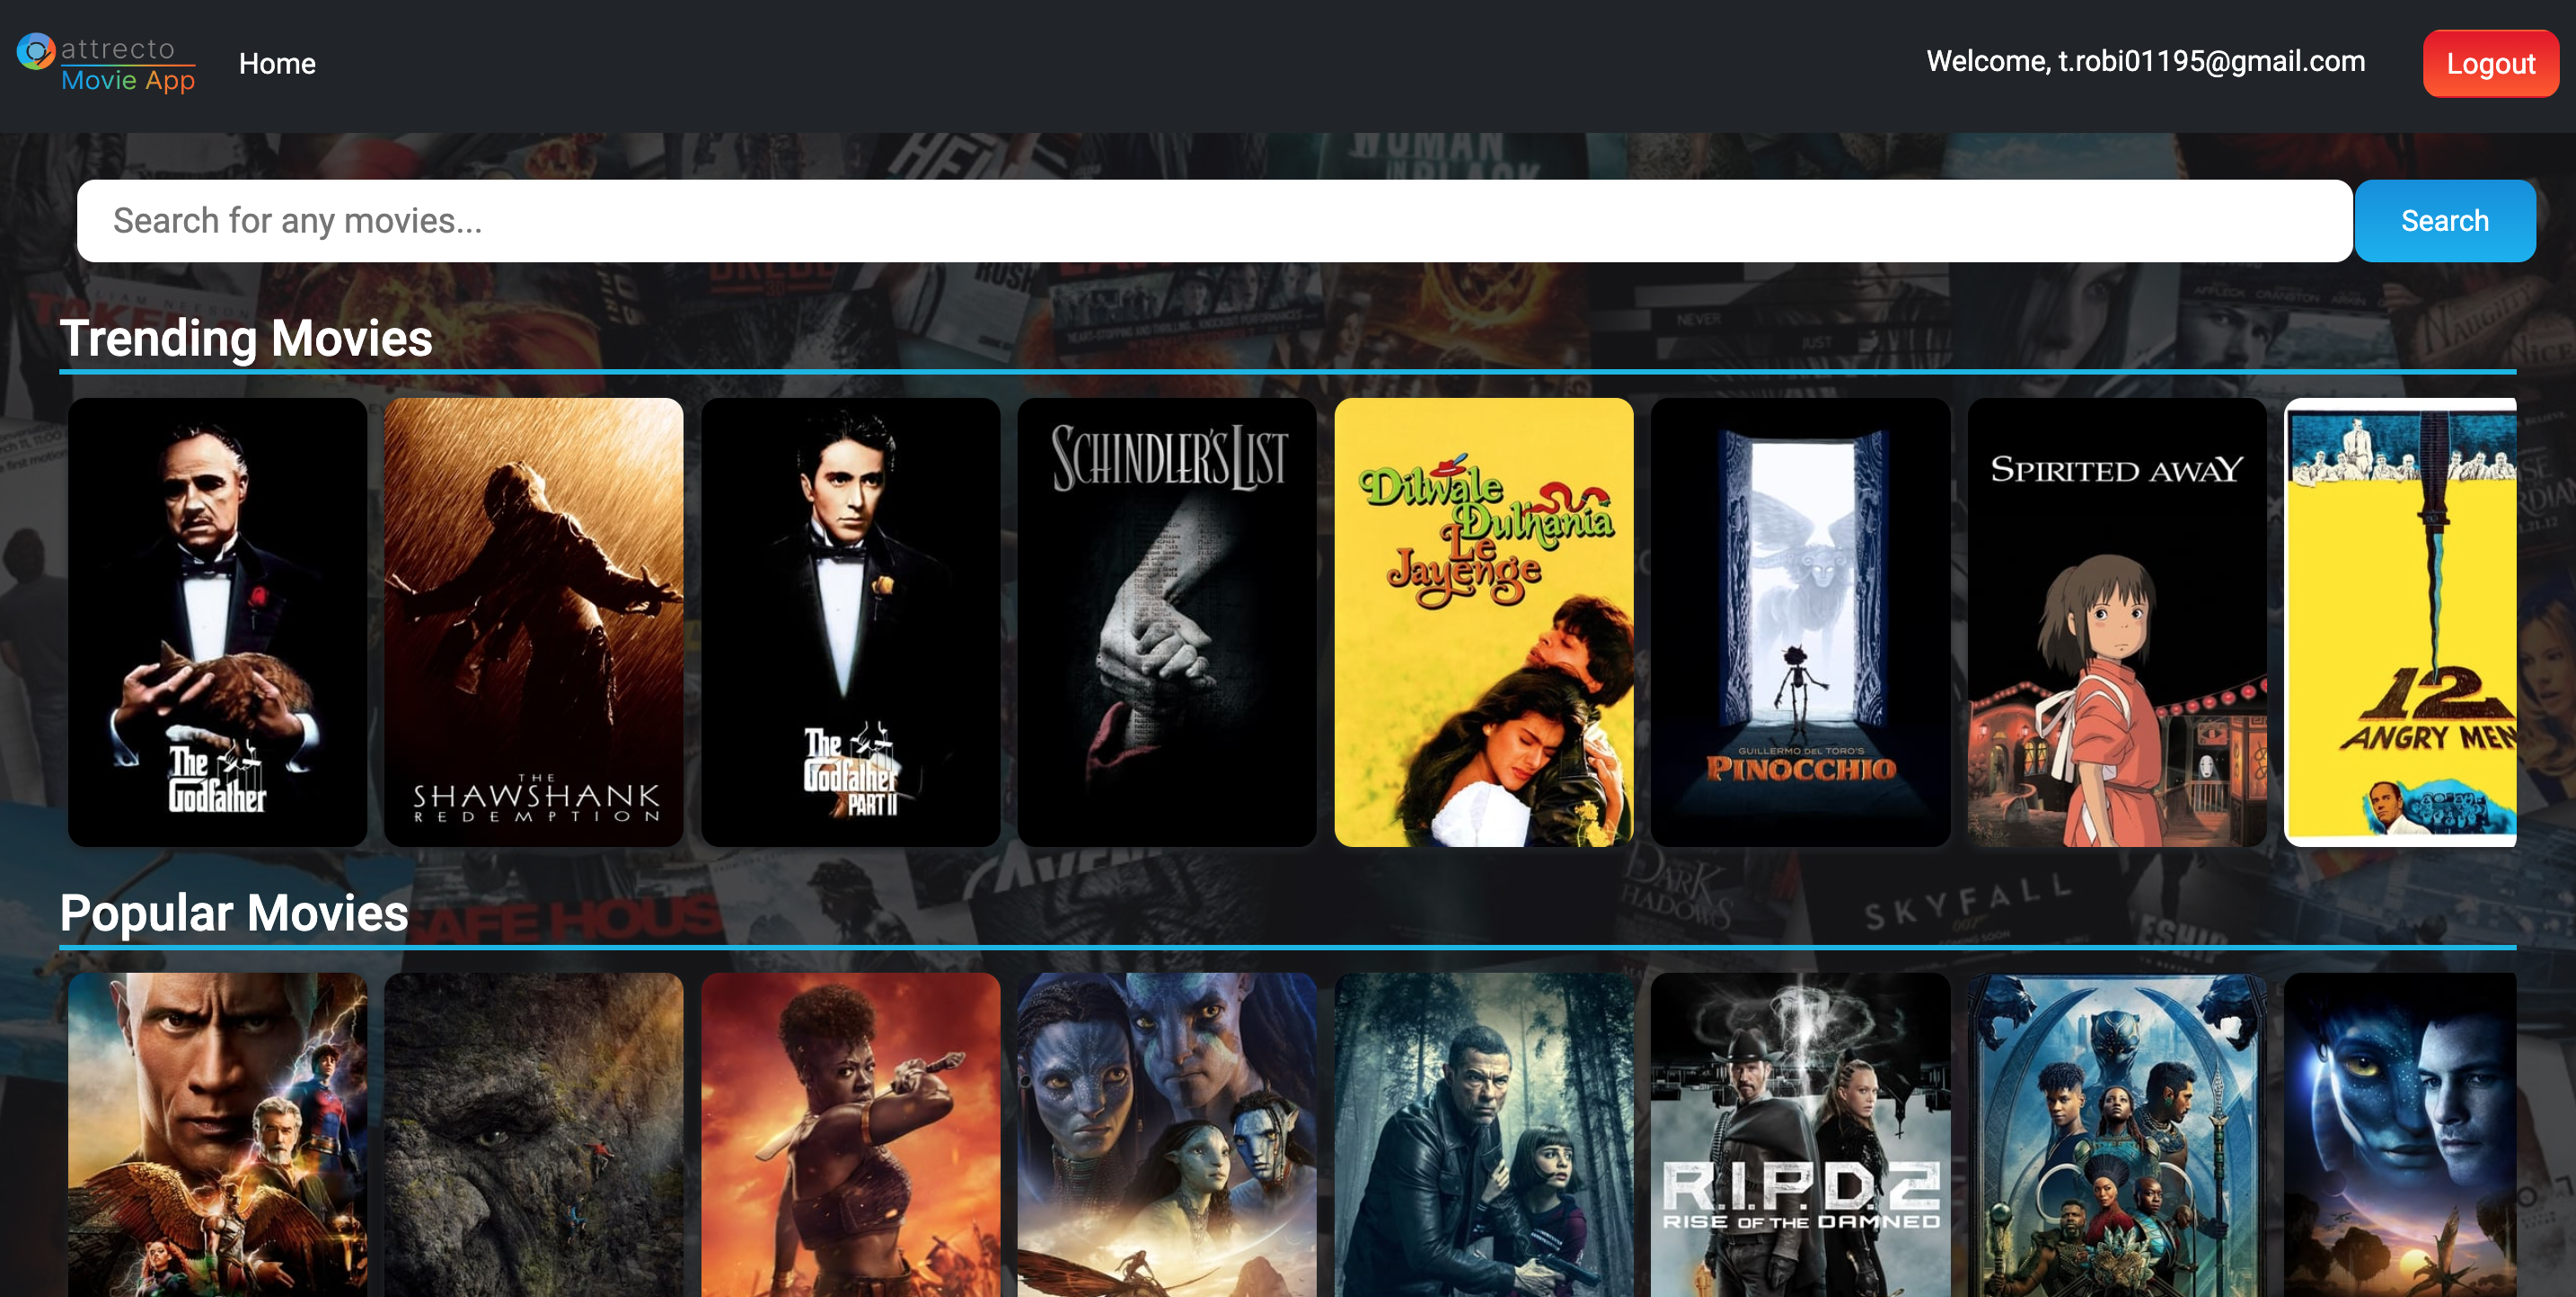
\includegraphics[width=140mm]{figures/movie-app.png}
    \captionsetup{labelformat=empty}
    \caption{Részlet a gyakornoki program feladatából}   
\end{figure}
\par A filmes gyakorlat után a többi gyakornokkal együtt részt vettem egy nagyobb projektben, ahol együtt dolgoztunk a vállalat belső weboldalának fejlesztésén. A fejlesztés sokkal nagyobb projekt volt, mint az előző gyakornoki alkalmak, ahol intenzíven használtam a Jira-t és a Confluence-t.
\par A projekt neve dashboard volt, amely egy olyan felület, amelyen a vállalat alkalmazottai különböző widgeteket helyezhetnek el tetszésük szerint. A webes alkalmazás Angular frontendre és több különböző backend technológiára (PHP, .NET stb.) épül, és mikrofrontend architektúrát használ minden egyes widgethez.
\par A kezdeti fázisokban a tervezés volt a fő hangsúly, a backend-fejlesztőkkel megbeszéléseket folytattunk a végpontokról és azok felépítéséről, majd a tervezés után elkezdtük az alkalmazás építését. Frontend oldalon az egyes feladatokat különböző widgetekre osztottuk, hogy könnyen, a fejlesztők közötti konfliktus nélkül fejleszthetőek legyenek.
\par A fejlesztés során az volt a feladatom, hogy létrehozzak néhány widgetet, miközben megtanultam a különböző könyvtárak használatát, a kódírást, a helyes programozási szokásokat és viselkedést, valamint a kód megfelelő formázását.
\section*{Összegzés}
\par Az Attrecto Zrt-nél töltött szakmai gyakorlatom során frontend fejlesztéssel foglalkoztam az Angular keretrendszer használatával, ahol megismerkedtem a HTML, JS és CSS technológiákkal, verziókezeléssel és projektmenedzsment eszközökkel. E munka során rengeteg tapasztalatot szereztem egy projekt lebonyolításának lépéseiről, valamint a kollégáimmal való kommunikációról és együttműködésről.



%\include{content/analizalas}
%\include{content/introduction}
%\include{content/thesis-format}
%\include{content/latex-tools}
%\include{content/template-usage}


% Köszönetnyilvánítás - opcionális
%~~~~~~~~~~~~~~~~~~~~~~~~~~~~~~~~~~~~~~~~~~~~~~~~~~~~~~~~~~~~~~~~~~~~~~~~~~~~~~~~~~~~~~
%\include{content/acknowledgement}


% Táblázatok listája - opcionális
%~~~~~~~~~~~~~~~~~~~~~~~~~~~~~~~~~~~~~~~~~~~~~~~~~~~~~~~~~~~~~~~~~~~~~~~~~~~~~~~~~~~~~~
%\clearpage\phantomsection
%\listoftables
%\addcontentsline{toc}{chapter}{\listtablename}


% Irodalomjegyzék
%~~~~~~~~~~~~~~~~~~~~~~~~~~~~~~~~~~~~~~~~~~~~~~~~~~~~~~~~~~~~~~~~~~~~~~~~~~~~~~~~~~~~~~
%\clearpage\phantomsection
%\bibliography{bib/mybib}
%\addcontentsline{toc}{chapter}{\bibname}


% Függelékek
%~~~~~~~~~~~~~~~~~~~~~~~~~~~~~~~~~~~~~~~~~~~~~~~~~~~~~~~~~~~~~~~~~~~~~~~~~~~~~~~~~~~~~~
%\include{content/appendices}

%\label{page:last}
\end{document}
